\begin{SCfigure}[1][htb]
    \centering
    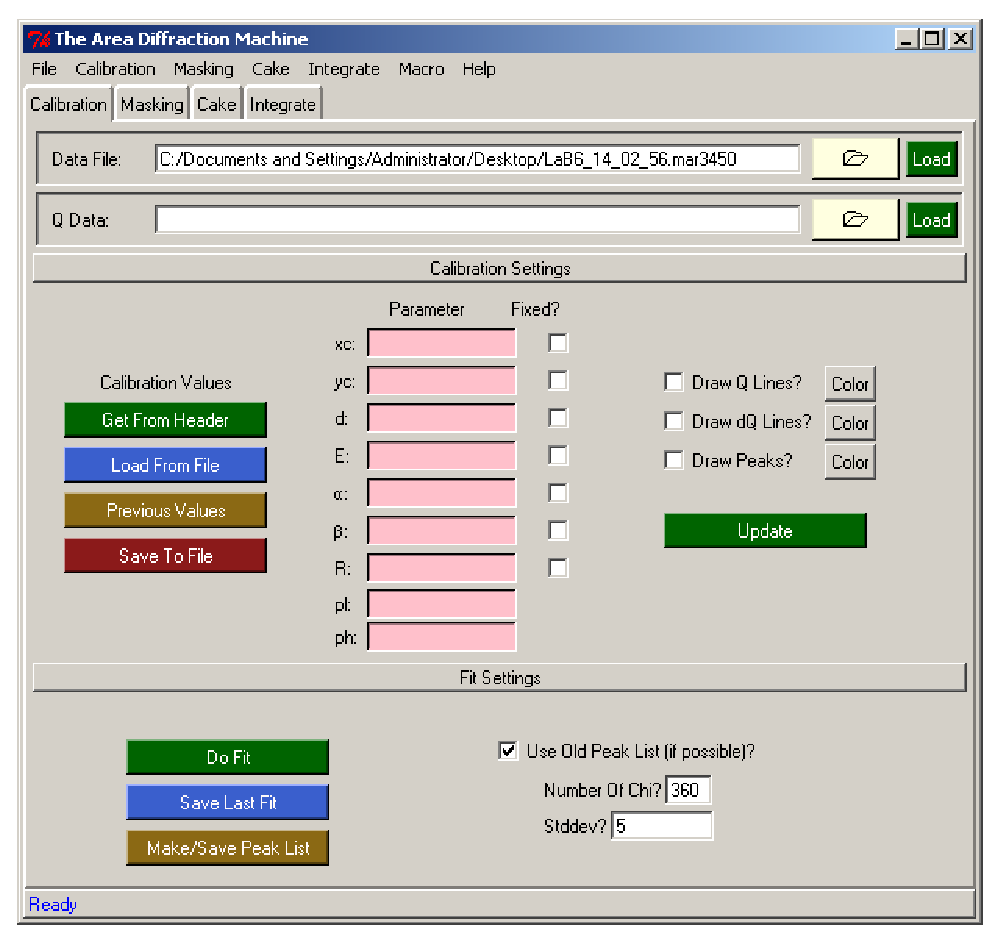
\includegraphics[scale=.75]{figures/calibration_tab.eps}
    \caption{A screen shot of the calibration tab.
    This is what you see when you first open the program. 
    This tab allows you to load diffraction
    data into the program.} 
    \label{calibration_tab}
\end{SCfigure}

When you first opep the Area Diffraction Machine, you
will see the calibration tab. It is shown in 
figure~\ref{calibration_tab}. The first thing you
will probably want to do is load diffraction data into
the program. This can be done with the \gui{Data File:} input
either by typin in the filename by hand and pushing the
load button or clicking on the folder icon and
using a file selector. After the file is loaded, a
diffraction data window will open. This window is 
shown in figure~\ref{diffraction_data_window}.

\begin{SCfigure}[1][htb]
    \centering
    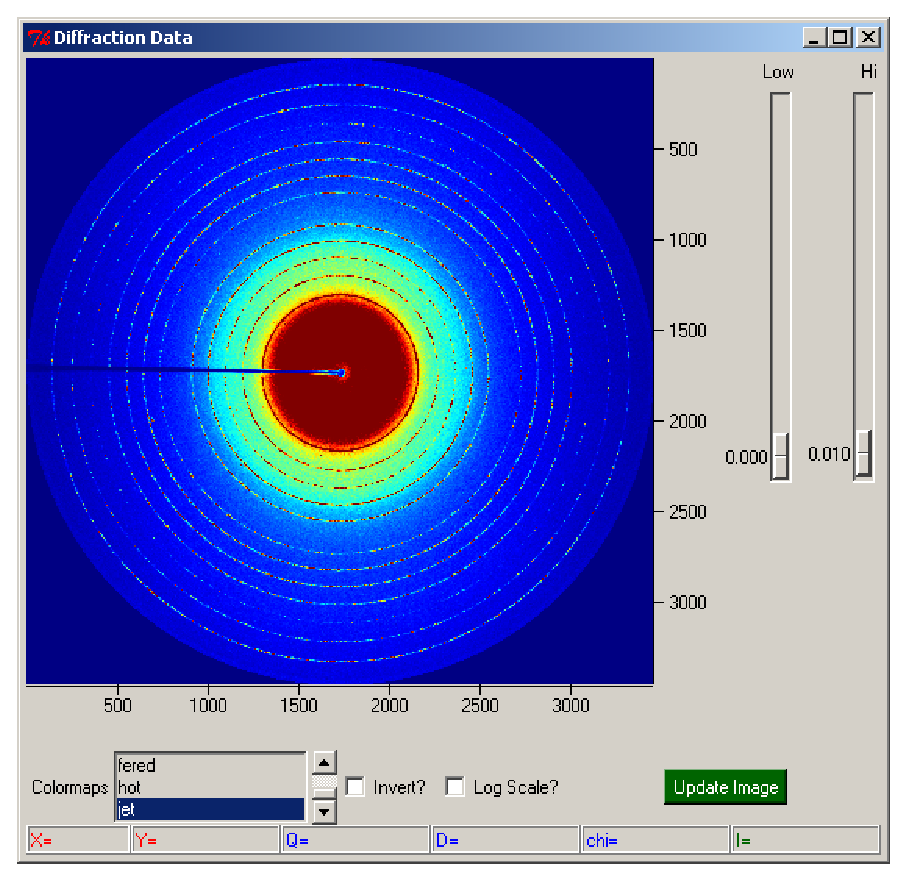
\includegraphics[scale=.75]{figures/diffraction_data_window.eps}
    \caption{A screen shot of the diffraction data window. This 
    window will open after a file is 
    loaded. This windows allows you to interact with diffraction 
    data.} 
    \label{diffraction_data_window}
\end{SCfigure}

You can use the diffraction data window to interact with your 
diffraction data. you can:
\begin{itemize}
    \item {\em Zoom into the data} -- left click on
    the data and hold down on the mouse. When you drag the cursor, 
    the program will create a resizing square. When you let go of the
    mouse, the selected square will be used as the outer bound and
    the image will be zoomed into it.
    \item {\em Zoom out of the data} -- right click on
    the data.
    \item {\em Pan across the data} -- hold shift, push down either mouse
    button, and then move the mouse around and the image will move 
    with it. Let go of the mouse to stop panning.
    \item {\em Resize the window} -- Click on the bottom right corner of
    the window and drag. The window will reszie just like any
    other program.  
    \item {\em Read coordinates for a selected point} -- When you
    mouse over the image, the $x$, $y$, $Q$, $\chi$, and $I$
    values for that pixel will be displayed at the bottom of the
    window. $Q$ and $\chi$ will only be dipslayed if valid calibration
    data is loaded into the program. See chapter~\ref{calibration}.
    \item {\em Change the Color Map} -- The \gui{Colormaps} selector 
    can be used to change the particular color map used to display the 
    data.
    \item {\em Invert the Color Map} -- The \gui{Invert?} checkbox can 
    can be used to invert the colors of the color map.
    \item {\em Low \& Hi Pixels} -- The sliders to the right of the 
    image can be used to change the intensity scaling of the
    image. The low value corresponds to the intenisty 
    value that will be maped to the lowest part of
    the color map and the hi value corresonds to the intensity
    value that will be mapped to the highest part of the color
    map. \footnote{Technically, what you actually set is what
    percentage of the most intense pixel in the image should be 
    mapped to the lowest or highest value in the color map.}
    This feature is useful because it can help make visible certain
    intensity ranges of the image.
    \item {\em Log Scaling} - By default, intensity values are linearly 
    mapped to colors in the color map. The \gui{Log Scale?} checkbox 
    can be selected to instead apply a log scale mapping of the intensity 
    values to the color map.
\end{itemize}

\section{File Formats}

The program can load in Mar data: \macroline{.mar2300}, 
\macroline{.mar3450}, and the \macroline{.mccd} Mar CCD format.
It can load in standard \macroline{.tiff} data. 
It can load in the ESRF Data Format \macroline{.edf}.
The program can only display square data. Whenever non-square
data is loaded into the program, the program will simply pad 
out the image until it is a square with pixels who's intensity is 0. 

\section{Loading Multiple Images}

Using the same file input, you can load multiple files into 
the program at the same time. If multiple files are put in 
the \gui{Data File:} text input  and separated by spaces, they
will all be loaded in. Alternately, the diffraction data file 
selector can be used to select multiple files at the same time.
All of the selected files will be loaded.
When several files are loaded at the same time, the program will 
add the intensities of the images pixel by pixel and work with the 
combined image.  This can be useful for analyzing several images 
taken of the same sample. The program can only add together files 
of the same format.

\section{Saving the Diffraction Image}
\index{Save}\index{ESRF Data Format}

You can save diffraction data in the program as a popular image format. 
The data can be saved by doing to the \gui{File} menu bar and selecting 
the \gui{Save Image} option.  The formats currently allowed are \gui{jpg}, 
\gui{gif}, \gui{eps}, \gui{pdf}, \gui{bmp}, \gui{png}, \gui{tiff}, and 
the ESRF data format \gui{edf}.

Images saved as a popular image format will be saved with whatever
threshold masks, polygon masks, $Q$ lines, $\Delta Q$ lines, and peaks 
are currently displayed over the data in the diffraction data 
window. And it will be saved at whatever the current zoom level 
is.\footnote{This is not the case with ESRF data. When an image
is saved as an ESRF file, it will be saved un-zoomed with none
of the lines or masks on top of it.} See chapter~\ref{calibration} for 
a discussion of the $Q$ lines, $\Delta Q$ lines, and peaks. See 
chapter~\ref{pixel_masking} for a discussion of threshold masks and 
polygon masks.

Because the program will pad any non-square data when
it is loaded to. The program will always save out 
all images as squares. If this is undesirable, the saved images
will need to be cropped using another program.

